%!TEX root = Constructive Alignment for Introductory Programming.tex

\chapter{Approaching Constructive Alignment with Portfolio Assessment} % (fold)
\label{cha:approach}

\graphicspath{{Figures/CAApproach/}}

\section{Guiding Principles} % (fold)
\label{sec:guiding_principles}

Our model for delivering constructive aligned introductory programming, presented in this chapter, is based upon the following principles. These principles acted as guidelines for decision making, and in many ways they underpin the model as intended learning outcomes underpin constructively aligned teaching. Each aspect of the model, the associated curriculum, teaching and learning activities, and assessment tasks are aligned with one or more of these principles.

The principles cover both \emph{how} the teaching and learning environment should operate, and \emph{what} should be taught. Originally derived from constructive alignment, the \emph{how} principles centre on constructivism and aligned curriculum. In relation to \emph{what} should be taught, the principles draw upon computing education literature and our own experiences as educators and software developers. Both sets of principles have developed over the course of this research through reflective practice.

\subsection{Principles for how the environment should operate} % (fold)
\label{sub:principles_for_how_the_environment_should_operate}

In the following list we outline the principles we used to guide our decisions on \emph{how} the teaching and learning environment should operate. These principles are general and could, therefore, be applied to a range of teaching and learning contexts and topic domains.

\begin{itemize}
	\item Recognise that students construct knowledge in response to activity.
	\item Align activities and assessment to intended learning outcomes.
	\item Aim to assess learning outcomes not learning pace or product outcomes.
	\item Focus on depth of understanding over breadth of coverage.
	\item Have high expectations of students.
	\item Actively support student efforts.
	\item Trust and empower students to control their own learning.
	\item Be agile and willing to change.
	\item Embed reflective practice in all aspects.
\end{itemize}

\subsubsection{Relationships between Principles} % (fold)
\label{ssub:relationships_between_principles}

Individually each principle has its own intrinsic value but they are designed to work together, in which case their effects multiply. Together, each principle interacts with the other principles to create a productive student centred learning environment.

\fref{fig:how_principles} shows the key interactions between these principles. The students active construction of knowledge is central, with various aspects of this being supported by the other principles. These various relationships will be discussed in the following sections.

\begin{figure}[htbp]
	\centering
	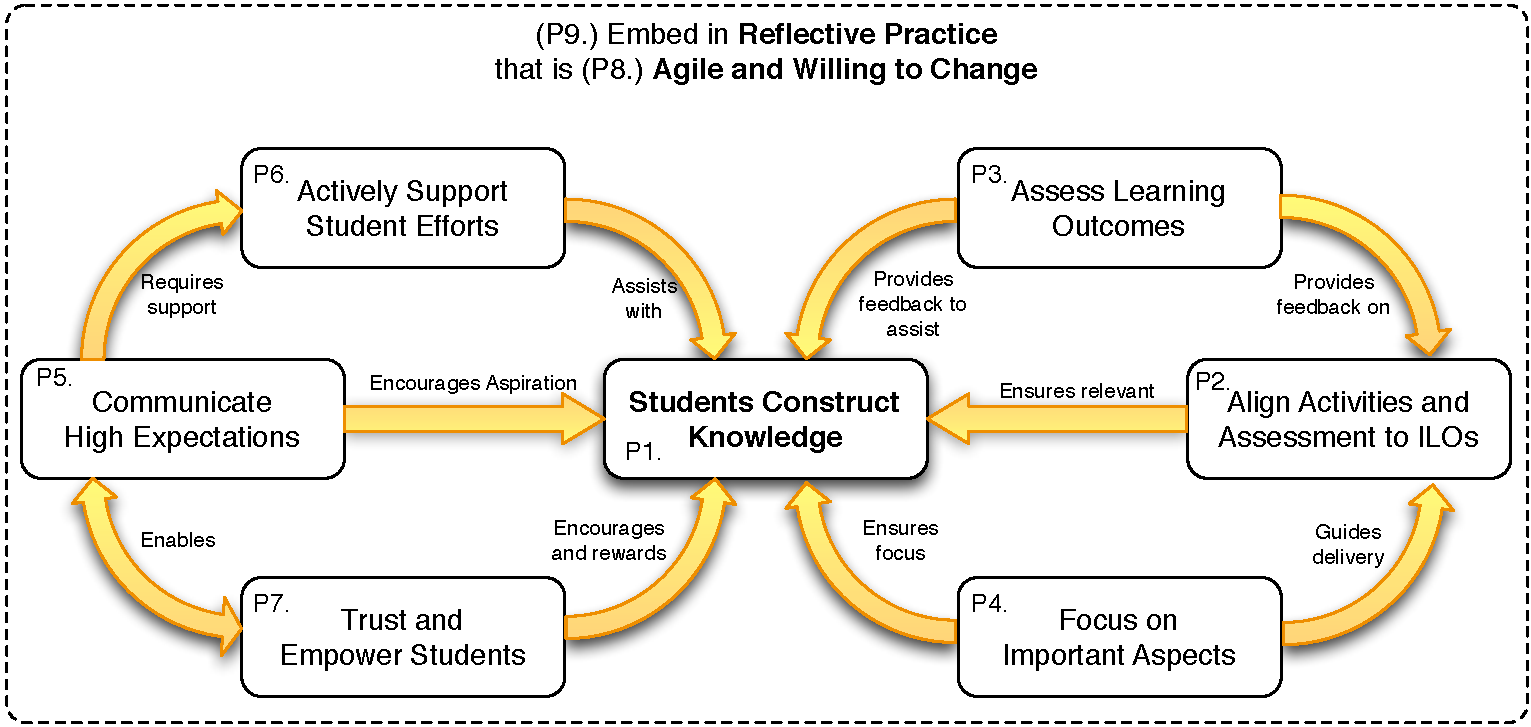
\includegraphics[width=\textwidth]{HowPrinciples}
	\caption{Key interaction between proposed principles.}
	\label{fig:how_principles}
\end{figure}

\subsubsection{Recognise that students construct knowledge in response to activity} % (fold)
\label{ssub:ideas_adopted_from_constructivism}

Decisions about curriculum, teaching and learning activities and assessment tasks are all guided by the educator's theory of teaching and learning \cite{Argyris:1976,Ramsden:1992}. While constructivism is often the espoused theory, \citet{Phillips:2005} indicates this has not transitioned to common education practice, resulting in a ``dissonance'' between the elements of effective learning and the characteristics of typical university learning environments. This is symptomatic of the disconnect between educators espoused theory and their theory-in-use \cite{Argyris:1976}. To successfully implement constructive alignment it will, therefore, be important to adopt the key aspects from constructivism outlined by \citet{Biggs:1996c}, \citet{Biggs:1997} and in \citet{Biggs:2007}. By consciously attempting to adopt constructivism as our theory-in-use we aim to create a educational setting which is ``in harmony'' with the principles of constructive alignment.

Central to all forms of constructivism is the principle that learning is an active process requiring the leaner to construct their own understanding through individual and social activity \cite{Biggs:1996c,Cunningham:1996,Duffy:1992,Glasersfeld:1989,Steffe:1995}. During the development of the model presented in this thesis we actively worked to embed the following aspects of constructivism in our theory-in-use.

\begin{itemize}
	\item Knowledge is constructed, not transmitted via communication alone.
	\item Teaching involves creating a context in which learns are able to construct appropriate cognitive models through individual and social activities.
	\item Errors in understanding are opportunities for further learning, these help indicate the students' current level of development and can be used to guide future learning activities.
\end{itemize}

\citet{Biggs:1996c} reason for adopting constructivism as a central philosophy was due to its emphasis on the students active role in constructing their own knowledge. When taken to an extreme this results in approaches that rely upon students building their own understanding from first principles, such as in discovery learning \cite{Bruner:1961}. These approaches are often promoted in constructivist writings, such as in \citet{Glasersfeld:1989} and \citet{Cunningham:1996}. The unstructured nature of these teaching and learning environments have received strong criticism. \citet{Anderson:1998} criticises constructive learning theories when ``pursued to unproductive extremes'', as in the case with discovery learning. \citet{Mayer:2004} argues against discovery learning, instead suggesting that constructivist views of education may be better served through cognitive activity, instructional guidance, and curricular focus. Furthermore, \citet{Kirschner:2006} argue against discovery learning indicating that in highly complex environment, such as with software development, free exploration may generate a heavy workload and detrimentally affect learning.

While we do take on board the central role of the learner in constructing their knowledge, we want to avoid detrimental aspects associated with taking these ideas to their extreme. As a result, we temper constructivism with certain practical details, an approach we feel is inline with the principles of constructive alignment. These details include the following:

\begin{itemize}
	\item Communication remains a valuable tool in helping shape the learning context.
	\item Guided instruction is valuable and ensures student activity is likely to be productive.
	\item Deliberate practice provides students with opportunities to engage with principles in action.
\end{itemize}

% subsection ideas_adopted_from_constructivism (end)

\subsubsection{Align activities and assessment to intended learning outcomes} % (fold)
\label{ssub:align_activities_and_assessment_to_intended_learning_outcomes_}

The second pillar of constructive alignment is aligned curriculum. The impact of aligning teaching and learning activities and assessment tasks was highlighted by \citet{Cohen:1987}. In discussing instructional alignment \citet{Cohen:1987} reported that the effect sizes based on achievement tests was up to four times greater than in non-aligned instruction. In proposing constructive alignment \citet{Biggs:1996c} aligns teaching and learning activities and assessment tasks to intended learning outcomes, weaving a ``web of consistency'' to optimise the likelyhood of students engaging appropriately with learning activities \cite{Biggs:1999}. 

In order to implement constructive alignment this ``web of consistency'' must also be achieved. The alignment of activities and assessment to intended learning outcomes will be critical for our model. As shown in \fref{fig:how_principles}, this alignment is seen as supporting student construction of knowledge. By aligning teaching and learning activities to the intended learning outcomes we ensure that students are constructing the required understanding. Similarly, by aligning assessment with these same intended learning outcomes we ensure that students are adequately prepared for this assessment and that the assessment is evaluating unit goals. 

% subsubsection align_activities_and_assessment_to_intended_learning_outcomes_ (end)


\subsubsection{Aim to assess learning outcomes not learning pace or product outcomes} % (fold)
\label{ssub:aim_to_assess_learning_outcomes_not_learning_pace_or_product_outcomes_}

Assessment in education is often seen as serving one of two purposes: supporting learning, or evaluating outcomes. These two purposes have come to be known as \emph{formative} and \emph{summative}, as proposed by \citet{Scriven:1967} and \citet{Bloom:1969}. To best support student construction of knowledge we want to maximise formative assessment. Using frequent formative feedback during the semester to aid students in developing appropriate understanding, and delaying summative assessment until after unit delivery.

To avoid assessing students pace of learning 100\% of each student's grade will be determined from the summative assessment. This ensures students are free to use the formative assessment to develop their understanding. As this work will not have marks attached students can highlight their misunderstandings and uncertainties without losing marks. We want to encourage students to use these formative tasks to demonstrate what they \emph{do not} know, as much as what they \emph{do}. 

Our assessment should, as much as possible, focus on providing feedback on student understanding and ability to meet the intended learning outcomes. We want to focus on more than just the ``product'' outcomes from the teaching and learning activities. Assessment tasks need to include aspects that require students to articulate their current understanding of concepts. This can then be used to help determine the students current level of understanding, and errors evident in this work provides opportunities for students to learn from their mistakes. 

%Traditionally programming units focus on code writing activities, and assessment then focuses on evaluating the programs produced. \citet{Lister:2004} augmented this with code reading and tracing activities to help better assess student understanding. We want to take this work further and assess, formatively and summatively, students ability to \emph{describe} and \emph{explain} underlying principles, code structures, and development processes. This will mean the code itself will be insufficient, and additional teaching and learning activities will need to get students to describe and explain aspects of software development.


This principle relates to both students construction of knowledge and to the alignment of activities and assessment, as shown in \fref{fig:how_principles}. Formative assessment of learning outcomes during delivery helps students in the construction of knowledge, providing opportunities to learn from their mistakes without fear of losing marks. These formative tasks also help both staff and students with the alignment of teaching and learning activities and assessment tasks. Staff can use these misunderstandings to help guide students individually, and to change or adjust teaching and learning activities where needed. For students, this ongoing focus on articulation of understanding and receiving feedback will ensure they are suitably prepared to demonstrate how they have met all of the intended learning outcomes in the final summative assessment.

The summative assessment also contributes to both students construction of knowledge and to the alignment of activities and assessment. For final unit grades students will need to demonstrate how their understanding aligns with the units intended learning outcomes. The assessment needs then to aim to assess the level of understanding demonstrated, in effect aiming to evaluate how suitable the students level of understanding is at the end of the unit.

Our position on the use of assessment in this way has significant support in the education research literature, with the value of feedback being widely reported. In proposing the use of formative assessment in education \citet{Bloom:1969} indicates that an assessment item can play both formative and summative roles, though he suggests that in this case the formative assessment will be less effective. \citet{Ramsden:1992} indicates that of all items on the Course Evaluation Questionnaire \cite{Ramsden:1991} the one that most clearly distinguished between the best and worst courses related to the provision of helpful feedback. \citet{Black:1998} show that substantial learning gains can be achieved by innovations designed to strengthen frequent feedback students receive. Furthermore, \citet{Black:1998} report that students pay more careful attention to feedback when there are no associated marks. In discussing assessment for learning \citet{Brown:2004} states that ``Formative feedback is critical'' and that ``feedback must be at the heart of the process'' if we are to make assessment an integral part of learning.

% \citet{Mattick:2007} identified the perceived lack of feedback as a barrier to creating a high quality learning environment for undergraduate medical students. 

The experience of \citet{Smith:2005}, however, indicates that shifting to formative assessment requires more than just removing the marks. \citet{Smith:2005} reported significantly worse results for the group of early secondary student who received only formative feedback. In discussing their results, \citet{Smith:2005} indicate that in this case comments were not often constructive, were misunderstood by students, and were not integrated back into the teaching and learning context. \citet{William:2006} indicates that to be formative, outcomes of the assessment must be used make adjustments to help students better meet learning needs. It appears that in the case examined by \citet{Smith:2005} the assessment remained primarily summative in nature with marks being replaced by comments. To be effective, our formative feedback must be communicated effectively to students and provide them with clear means of addressing any shortcomings.

\citet{Gibbs:2004} lists ten conditions under which assessment assists with student learning, shown below. The design of our model needs to ensure that all of these conditions can be met.
\begin{enumerate}
	\item Sufficient assessed tasks are provided for students to capture sufficient study time.
	\item These tasks are engaged with by students, orienting them to allocate appropriate amounts of time and effort to the most important aspects of the course.
	\item Tackling the assessed task engages students in productive learning activity of an appropriate kind.
	\item Sufficient feedback is provided, both often enough and in enough detail.
	\item The feedback focuses on students' performance, on their learning and on actions under the students' control, rather than on the students themselves and on their characteristics.
	\item The feedback is timely in that it is received by students while it still matters to them and in time for them to pay attention to further learning or receive further assistance.
	\item Feedback is appropriate to the purpose of the assignment and to its criteria for success.
	\item Feedback is appropriate, in relation to students' understanding of what they are supposed to be doing.
	\item Feedback is received and attended to.
	\item Feedback is acted upon by the student.
\end{enumerate}

% subsubsection aim_to_assess_learning_outcomes_not_learning_pace_or_product_outcomes_ (end)

\subsubsection{Focus on depth of understanding over breadth of coverage} % (fold)
\label{ssub:focus_on_depth_of_understanding_over_breadth_of_coverage_}

With limited resources, primarily time, the classic depth-vs-breadth trade off needs to be considered. Given that we have fixed time, we can either focus on providing a breadth of coverage, or a depth of understanding. 
As programming is central to the discipline of computing \cite{McGettrick:2005}, it will be important to focus on building depth of understanding.

The study conducted by \citet{Schwartz:2009} found that high school students who reported studying a major topic in depth earned higher grades in college than those who reported covering no topics in depth. If this can translate to undergraduate computing education, then a depth of understanding in programming may help students succeed with other computing units. Given the strong correlation generally observed between programming skills and other computing skills \citet{McGettrick:2005} this is likely.

Depth over breadth will help focus the teaching and learning activities and assessment tasks, and ensure that they align to sufficiently deep cognitive levels. As the tasks define what students will do, this will in turn help ensure that students are developing appropriately deep knowledge in relation to the intended learning outcomes.

% subsubsection focus_on_depth_of_understanding_over_breadth_of_coverage_ (end)

\subsubsection{Have high expectations of students} % (fold)
\label{ssub:have_high_expectations_of_students_}

Believing in students' potential and communicating high expectations will be important in the development of the model. In listing their principles for good undergraduate education \citet{Chickering:1987} include communicating high expectations as one of their seven principles. \citet{Chickering:1987} state ``expect more and you will get more'' and indicate that high expectations are important for everyone, from those who are poorly prepared or unwilling to exert themselves to those who are bright and motivated. Believing in students' potential is also key to the approach presented by \citet{Soetanto:2003,Soetanto:2012}. Soetanto's approach aims to improving students' discipline, confidence and belief in their potential and technical units delivered with this approach have gained in popularity despite their technical difficulty and being delivery in a foreign language (English).

By having high expectations of our students we hope to build student confidence and get them to aspire to excellence. These expectations will then require students to work hard throughout the unit's delivery, providing encouragement to spend sufficient time on the teaching and learning activities. This will require both time and energy from students, which should improve outcomes: as stated by \citet{Chickering:1987} ``time plus energy equals learning''.

% subsubsection have_high_expectations_of_students_ (end)

\subsubsection{Actively support student efforts} % (fold)
\label{ssub:actively_support_student_efforts}

Both \citet{Chickering:1987} and \citet{Soetanto:2003,Soetanto:2012} indicate high expectations should also apply to teaching staff. If we are to reasonably expect a lot from our students, they should expect a lot from us. To help students achieve the required understanding we need to actively support their efforts. This will need to extend beyond providing formative feedback, to providing active support throughout the process. Given the technical nature of introductory programming and the exacting nature of compiler, students are going to face numerous challenges. Learning to program \textbf{is} hard, so we must make every effort to support our students.

% subsubsection actively_support_student_efforts (end)

\subsubsection{Trust and empower students to control their own learning} % (fold)
\label{ssub:trust_and_empower_students_to_control_their_own_learning}

Student motivation has a significant impact on learning. In terms of strategies for improving student motivation, \citet{McGregor:1960} work on motivational strategies in business provide some insights into similar strategies that could be applied to education.  In his work on personnel management, \citet{McGregor:1960} identified two means of categorising how managers perceived their employees named Theory X and Theory Y. Traditionally businesses were seen to use coercion or persuasion as a strategy to motivate employees to achieve required levels of productivity. These strategies are used when managers adopt the view that employees do not want to work and cannot be trusted, \citet{McGregor:1960} named this understanding of human motivation as Theory X. In contrast, Theory Y assumes that, given the right conditions, people want to work, that they can be trusted and will do their best work when they are.

While applied to business organisation management, these two views can also be applied to an educational setting. \citet{Biggs:2007} argues for the adoption of Theory Y climates to get the most out of students. This is supported by \citet{Markwell:2004} who categorises Theory X teaching environments as ones where teachers assume that:

\begin{itemize}
	\item Students have little desire to learn new material.
	\item Students are inherently lazy and will attempt to get the material dumbed-down; the teacher must use a controlling environment to force students to learn and prevent cheating.
	\item Students prefer to be directed and do not want to be responsible for their own learning.
	\item The teacher must act as the source of information and actively transmit it to the students.
	\item Many students are not capable of learning the necessary material and can be expected to earn a low grade.
\end{itemize}

\noindent This is in contrast to list provided by \citet{Markwell:2004} for Theory Y environments where teachers assume that:

\begin{itemize}
	\item Learning is as natural to students as play or rest.
	\item Students are not lazy; threats of diminished grades are not necessary to motivate students.
	\item The self-satisfaction from learning is sufficient to commit students to achieving the educational objectives.
	\item Students will naturally accept responsibility for learning.
	\item Imagination, ingenuity, and creativity are widely distributed within the student population and will be willingly applied to the learning process.
	\item The intellectual potential of most students are being only partially utilized in the classroom.
\end{itemize}

In order to achieve many of the principles listed here it will be necessary for us to adopt a predominantly Theory Y stance. The formative nature of the assessment tasks together with the high expectations will both require a level of trust in students that cannot be achieved with a predominantly Theory X stance. High expectations of students is a natural repercussion of Theory Y, and enhancing motivation in this way should help students in the construction of their knowledge.

% subsubsection trust_and_empower_students_to_control_their_own_learning (end)

\subsubsection{Embed reflective practice in all aspects} % (fold)
\label{ssub:embed_reflective_practice_in_all_aspects}

In education the idea of reflective practice is to periodically look back at our teaching, and consider how things can be improved. The foundations of this idea can be traced back \citet{Dewey:1933}, though reflective practice was originally proposed by \citet{Schon:1983}. \citet{Farrell:2007,Farrell:2008} identify two forms of reflective teaching practice: a strong form and a weak form. In its weak form, reflective practice involves informal evaluation of various aspects of professional practice. \citet{Farrell:2008} likens this to no more than thoughtful practice. The alternative strong form of reflective practice involves systematic reflect on teaching and taking responsibility for teaching and learning activities. To ensure ongoing improvements, the model we propose needs to incorporate reflective practice. We propose to user reflective teaching ``hand-in-hand with critical self-examination and reflection as a basis for decision making, planning, and action'' \cite{Richards:1994}. % (p.ix)

From a practical perspective, we can use common misconceptions identified in formative feedback to update delivery during the semester. After the semester, we can use students' results, both in terms of grade distributions and quality of evidence demonstrated in the final summative assessment, to suggest changes for following iterations. Reflections on teaching should be shared amongst all teaching staff related to the unit to provide them with an opportunity to reflect on their practice, and to enable them to learn from each other.

Reflective practice also needs to be encouraged in the student body. Students undertaking units taught with this approach will graduate and move into professional practice. Engaging them with reflective practice throughout their education will help ensure they are adequately equipped to engage in lifelong learning \cite{Field:2006}. The active incorporation of frequent formative feedback will provide a direct means of encouraging students to reflect on their work throughout the delivery of the unit. To further encourage reflection, their summative assessment should include some reflective aspects where they can reflect on what they have achieved in the unit. 

Reflection underpins all of the principles presented. Students engage in reflection as a tool to help them construct their knowledge, and the formative feedback enables student and staff reflections. Staff will reflect on teaching and learning activities, their alignment to learning outcomes, and the depth and breadth of coverage. Reflections will enable us to realistically manage expectations, the support we offer students, and to help us balance trust with mechanisms to avoid exploitation. Even the nature and composition of these principles have been the focus of our ongoing reflective practice.

% subsubsection embed_reflective_practice_in_all_aspects (end)


\subsubsection{Be agile and willing to change} % (fold)
\label{ssub:be_agile_and_willing_to_change}

For reflective practice to actively enhance our teaching we must embrace change, focusing on aspects that will deliver the most value for students for the effort required. As software developers, this emphasis on delivering value by focusing on the things that matter most was reminiscent of the agile software development principles \cite{Martin:2003}. The Agile Manifesto \cite{Beck:2001} laid down several key values: 

\begin{itemize}
	\item Individuals and interactions over processes and tools
	\item Working software over comprehensive documentation
	\item Customer collaboration over contract negotiation
	\item Responding to change over following a plan
\end{itemize}

\noindent To realise all of these principles it will be necessary to adopt similar values in our teaching, valuing things that help students construct their knowledge over other activities.

To help manage change effectively we view the environment as consisting of an underlying strategy, teaching and learning resources, and teaching and learning activities as shown in \fref{fig:strategy}. The strategy relates to the overall plan for delivering the unit content and informs the development of the intended learning outcomes. The central role of the intended learning outcomes means that the overall strategy should not change unless significant issues are identified in the approach overall. Teaching and learning resources and activities can then be separated to enable the development of reusable resources, meaning that activities can be adjusted more freely to better help them direct student efforts. The details of this are summarised in the following list.

\begin{figure}[htbp]
	\centering
	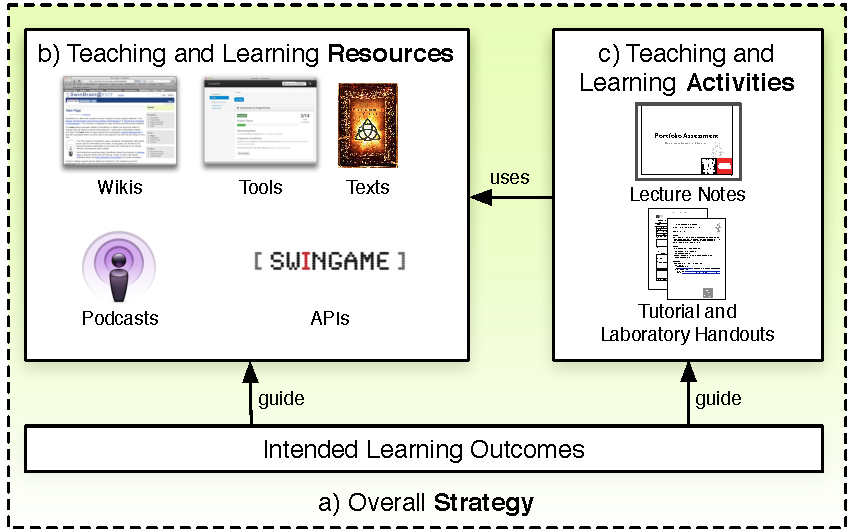
\includegraphics[width=0.8\textwidth]{StrategyResourcesActivities}
	\caption{Relationship between strategy resources and activities.}
	\label{fig:strategy}
\end{figure}

\begin{itemize}
	\item Develop an overall \emph{strategy} for delivering the unit content.
	\begin{itemize}
		\item Derive intended learning outcomes from the strategy.
		\item Use strategy to focus other teaching and learning resources and activities.
		\item Avoid changing strategy, unless approach has significant issues.
	\end{itemize}

	\item Create teaching and learning \emph{resources}.
	\begin{itemize}
		\item Deliver material following the direction from the overall strategy.
		\item Make resources generic and self contained.
		\item See as providing a supporting role to the teaching and learning activities.
		\item Invest in initial development, actively reuse and enhance over time.
		\item Improve integration with delivery material as resources prove to be effective.
	\end{itemize}

	\item Design teaching and learning \emph{activities}.
	\begin{itemize}
		\item Use these to focus student activity.
		\item Actively review each semester, and rework based on reflection.
	\end{itemize}
\end{itemize} 

% subsubsection be_agile_and_willing_to_change (end)


\subsubsection{Related Work on Education Principles} % (fold)
\label{ssub:related_work_on_education_principles}



\citet{Chickering:1987} list seven principles for 
\begin{enumerate}
	\item Encourages Contact Between Students and Faculty.
	\item Develops Reciprocity and Cooperation Among Students
	\item Encourages Active Learning
	\item Gives Prompt Feedback
	\item Emphasizes Time on Task
	\item Communicates High Expectations
	\item Respects Diverse Talents and Ways of Learning
\end{enumerate}



% subsubsection related_work_on_education_principles (end)

% subsection relationships_between_principles (end)



% subsection principles_for_how_the_environment_should_operate (end)

Principles specific to teaching introductory programming are presented in the following list. While the general principles helped shape the overall learning environment, these principles helped shape specifics in the curriculum, teaching and learning activities, and assessment tasks.

\begin{itemize}
	\item Focus on programming concepts.
	\item Introduce programming concepts incrementally, building on earlier concepts.
	\item Treat syntax as a means of expressing programming concepts, mapping conceptual programs to code for the compiler.
	\item Use the language as it is intended to be used.
	\item Avoid language features before they can be explained.
	\item Introduce concepts early and provide students with time to put them into practice.
	% \item Program code is not, by itself, a suitable means of measuring learning outcomes.
\end{itemize}

Each of these principles is expanded upon in the following sections, and linked to associated research.






\subsection{Supporting Student Learning} % (fold)
\label{sub:supporting_student_learning}

High Expectations: strive for excellence, responsibility for learning, be proud of their achievements.

\citet{Chickering:1987}:

\citet{Gibbs:2004} 

\begin{quote}
	The trick when designing assessment regimes is to generate engagement with learning tasks without generating piles of marking.
\end{quote}

% subsection supporting_student_learning (end)


\subsection{Adopted Principles} % (fold)
\label{sub:adopted_principles}


% subsection adopted_principles (end)



% section guiding_principles (end)

\section{Teaching Philosophy} % (fold)
\label{sec:teaching_philosophy}

\begin{itemize}
	\item Assess outcomes, not pace of learning
	\item Facilitate learning 
	\item Cultivate a climate that values understanding
\end{itemize}



% section guiding_principles (end)

\section{Implications} % (fold)
\label{sec:implications}

% section implications (end)

\section{Implementation} % (fold)
\label{sec:design}

Constructive alignment, as proposed by Biggs~\cite{Biggs:1996c}, is an amalgamation of constructive learning theory and aligned instruction design. It aims to elicit deep learning approaches from all students. Biggs' model is student focused, with clear and intentional alignment of assessment, teaching and learning activities, and unit objectives. The focus on the central role of the learner in building meaning is derived from constructivist learning theories, whilst the alignment of assessment, teaching, and learning activities, has its foundation in instructional design literature. 

\fref{fig:constructive_alignment} illustrates the constructive alignment model presented in~\cite{Houghton:2004}, which consists of the following blocks:

\begin{itemize}
	\item \emph{Intended learning outcomes} clearly define required learning in terms of ``performances of understanding''.
	\item \emph{Performance objectives} emerge from the desired outcomes, and can be ranked to become the assessment criteria.
	\item \emph{Teaching and learning activities} are designed to place students in situations likely to elicit the required learning.
	\item Students provide \emph{evidence of their learning}, that is assessed against the criteria to determine grade outcomes.
\end{itemize}

% \begin{figure}[t!]
% 	\centering
% 	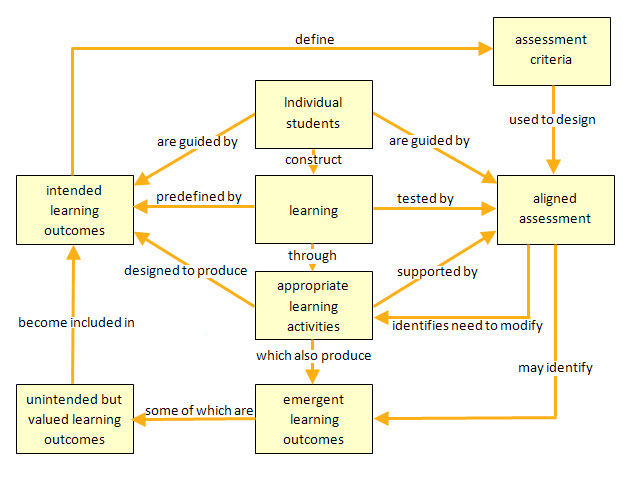
\includegraphics[width=\columnwidth]{Houghton_constructive_alignment_1}
% 	\caption{Constructive alignment model presented by Houghton in~\cite{Houghton:2004}}
% 	\label{fig:constructive_alignment}
% \end{figure}

The first stage of our research was to determine how Biggs' model of constructive alignment~\cite{Biggs:1996c}, and the details on using portfolio assessment suggested by Biggs and Tang in~\cite{Biggs:1997}, could be used to guide the creation of an introductory programming unit. Examining the practical advice from Biggs and Tang in~\cite{Biggs:2007}, which further elaborates on both his model of constructive alignment and portfolio assessment, a model of constructive alignment for introductory programming was defined. The model is presented in \fref{fig:process_overview}, which captures staff and student processes and the artefacts generated and exchanged throughout the learning process.

\begin{figure*}[t!]
	\centering
	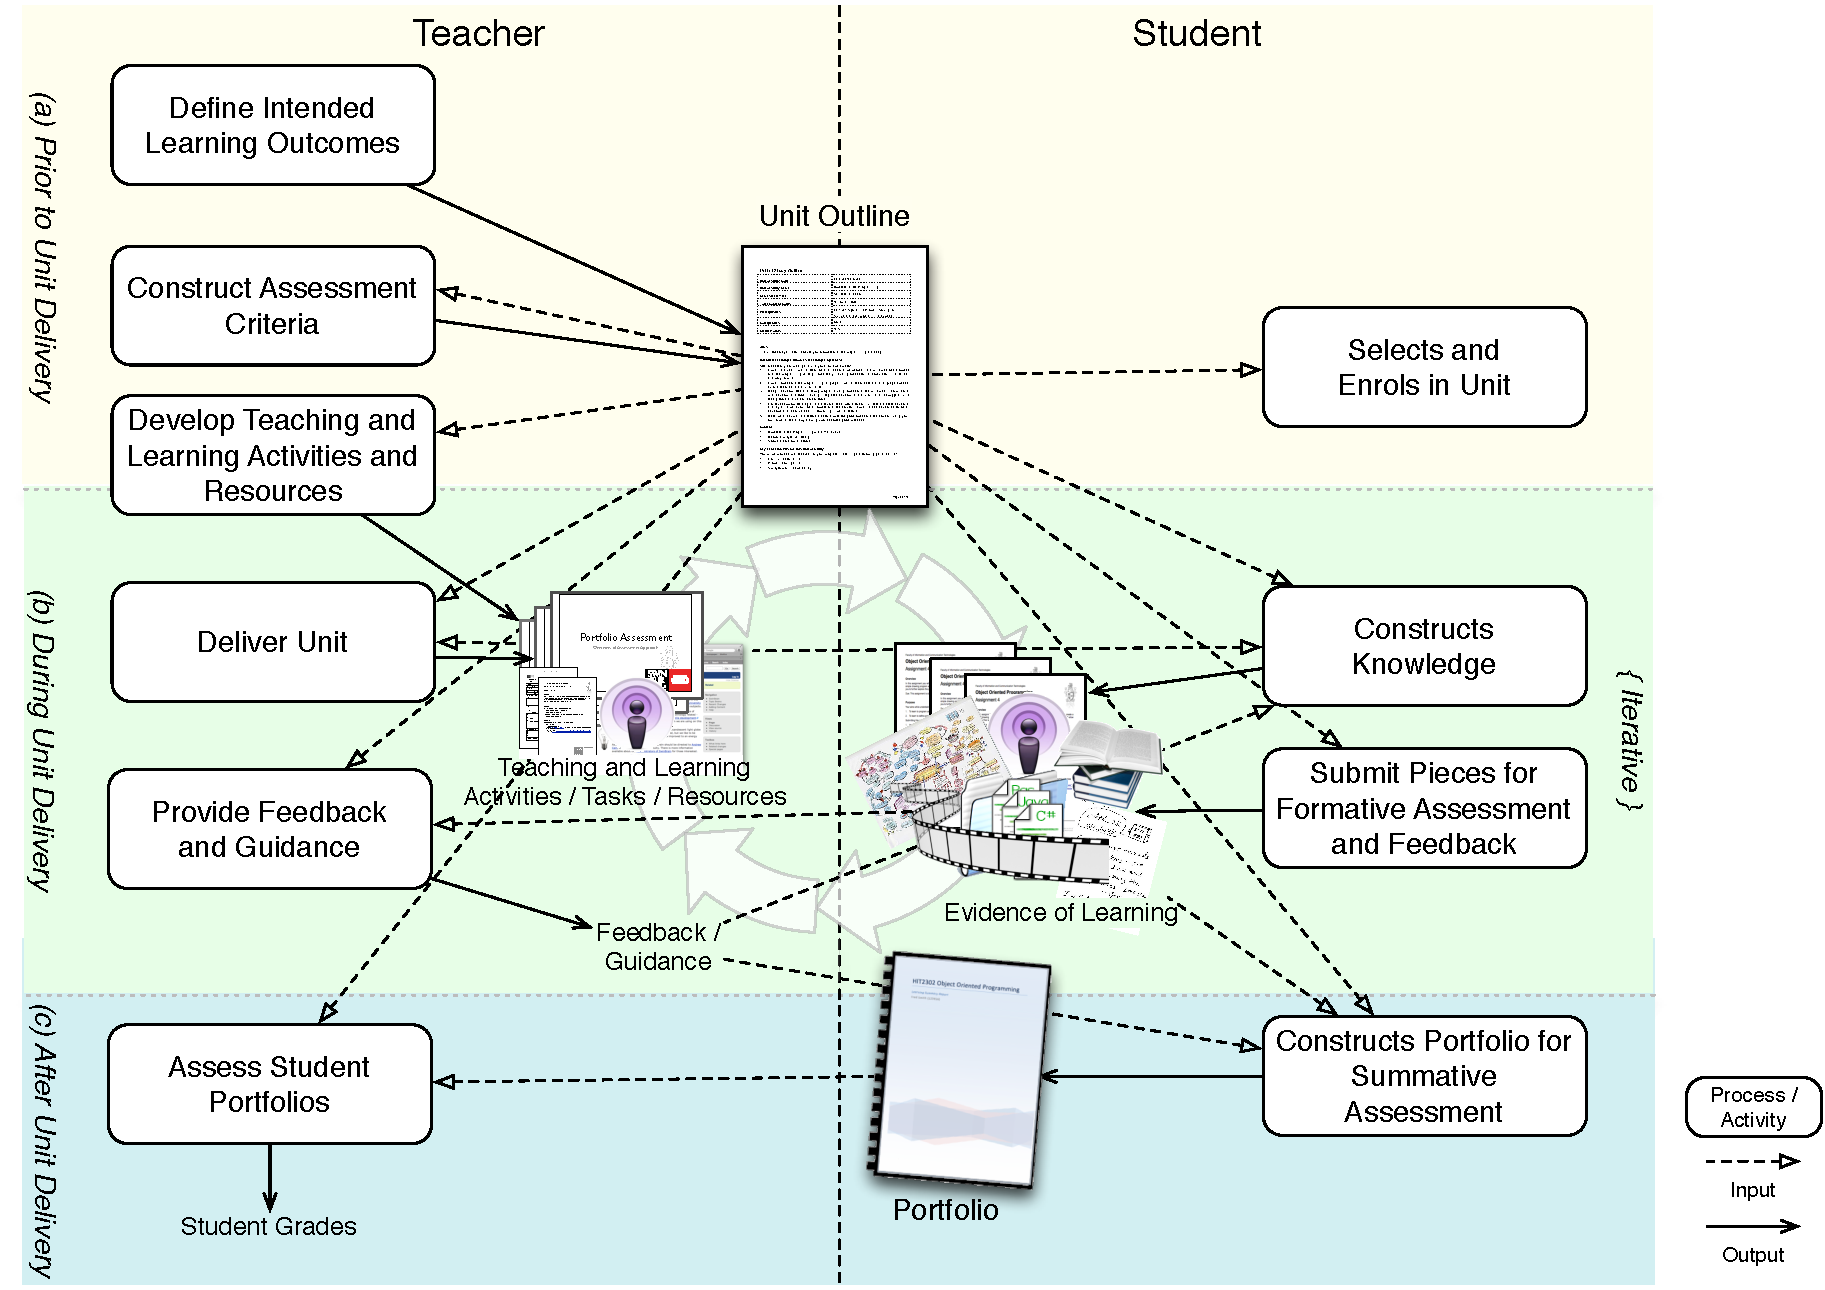
\includegraphics[width=6in]{ProcessOverview}
	\caption{An overview of teacher and students roles, and iterative delivery, in the constructive alignment model developed for introductory programming.}
	\label{fig:process_overview}
\end{figure*}

The model is divided into \emph{student} and \emph{teacher}\footnote{Teacher in this context encompasses all teaching staff related to the unit, though each stage may not involve all staff members.} processes, distributed throughout unit design and delivery. This is highlighted in \fref{fig:process_overview} by columns for the teacher and student processes, and three rows for the stages in which they occur. The stages identified are \emph{prior} to unit delivery, \emph{during} unit delivery, and \emph{post} unit delivery.

Prior to the unit delivery (a) the teaching staff \emph{define intended learning outcomes} and \emph{construct assessment criteria}, which together form the critical components of the unit outline. Such a document is a common practice, and forms the central focus for the unit. The unit outline is then used to inform and guide staff in the \emph{development of teaching and learning activities}. Unit outlines may also be used by students in evaluating units to select in their course.

During the teaching period (b), staff \emph{deliver the unit} using the developed teaching and learning activities. Ideally these activities help student's to \emph{construct knowledge}. As a result, students produce artefacts that demonstrate their depth of understanding, which may then be selected by the student and \emph{submitted for formative feedback}. This provides an opportunity for teaching staff to \emph{provide feedback and guidance}. The process of activities, knowledge construction, and formative feedback is designed to be an ongoing iterative process.

After the delivery of the unit (c) students \emph{construct and submit a portfolio for assessment}, which is then \emph{assessed by} the teaching staff against the intended learning outcomes and assessment criteria prepared prior to the unit's delivery.

The central role of intended learning outcomes and assessment criteria is to, as Biggs elegantly phrased it, ``entrap'' students ``in this web of consistency, optimising the likelihood that they will engage the appropriate learning activities.''~\cite{Biggs:1999}

While each of the processes described is important, some are of more interest than others when defining a constructively aligned approach. Of specific interest is the definition of the intended learning outcomes, the setting of the assessment criteria, the use of formative feedback during delivery, and the assessment of the portfolio.

\section{Model Process Details} % (fold)
\label{sec:process_details}

Here we outline the different processes of the model presented, with supportive examples from an initial implementation. The model was applied to a second level programming unit that focused on object oriented programming. Students are assumed to have been previously introduced to procedural programming, and as such were expected to have a working understanding of basic programming constructs (sequence, selection, repetition), as well as function and procedure declarations and parameter passing. 

The goals of the second programming unit were to introduce students to objects, object oriented principles, responsibility driven design, and to develop proficiency using an object oriented programming language. In this early example of the model's application, the unit was taken by 83 students and taught by a small team of staff. The model has been subsequently adapted and applied to other introductory programming units which are not dissimilar, though not discussed in this paper.

\subsection{Defining Intended Learning Outcomes} % (fold)
\label{sub:defining_intended_learning_outcomes}

When using constructive alignment, the intended learning outcomes are central to the assessment of the unit. With more \emph{traditional} forms of assessment, teaching staff take responsibility for aligning assessment to required outcomes. With portfolio assessment, teaching staff relinquish control of this aspect and the outcomes themselves take on a dual purpose: as a statement of what will be \emph{taught}, and what will be \emph{assessed}. Effectively the specified unit outcomes become the assessment, thereby taking advantage of the fact that ``assessment always drives the curriculum'' (Ramsden~\cite{Ramsden:1992}).  In this arrangement there is little opportunity for misalignment between the unit objectives and assessment, but a greater importance on the exact nature of the intended learning outcomes. This critical role of the intended learning outcomes means that they are instrumental in the success of the unit. 

For an introductory programming unit it is important to design the intended learning outcomes so that, as a group, they cover the required programming competencies as well as the associated conceptual knowledge. As the outcomes drive the entire process -- including both student and teacher processes -- it is important they are expressed clearly and simply so as to be understood by all involved.

A variety of sources serve as inputs into this process, though these are not shown in \fref{fig:process_overview}. In preparing learning outcomes, Thota and Whitfield propose inputs related to pedagogic theory (constructivism and phenomenography) as well as student factors such as approach to learning, learning styles, and prior knowledge. Armarego~\cite{Armarego:2009} highlights the needs for input related to industry requirements and domain characteristics, such as the Computer Science and Software Engineering Curriculum from professional standards bodies (see~\cite{Lethbridge:2006} and~\cite{Cassel:2008}), and associated Bodies of Knowledge (see~\cite{Abran:2001}).

We developed the following principles which can be used to guide the formation of the intended learning outcomes for portfolio assessed programming units:
\begin{itemize}
  \item Express outcomes using verbs at an appropriate level of understanding with reference to the SOLO taxonomy. (See~\cite{Biggs:2007} and~\cite{Biggs:1982}.)
  \item Cover both the required \emph{conceptual knowledge}, and \emph{programming competencies}.
  \item Use \emph{simple terms} (where possible) to communicate outcomes, ensuring they are understood by all students undertaking the unit.
  \item The number of outcomes should be \emph{minimal}, ideally between four and six (\emph{cf.}~\cite{Biggs:2007} and~\cite{Gardner:1994}). This is to help ensure that each outcome covers a meaningful body of knowledge to a sufficient depth.
  \item Outcomes need to be \emph{general} to facilitate assessment of diverse portfolios, and \emph{sufficient} to ensure that differing degrees of proficiency and understanding can be assessed.
  \item There needs to be \emph{flexibility} to enable students to choose a range of means when addressing outcomes.
\end{itemize}

In the example implementation presented in this work, the learning objectives had been predefined, as required by the outside influence of accreditation processes, but were expressed using appropriate action verbs. \tref{tbl:example_intended_learning_outcomes} lists the outcomes from the example unit delivered using this model.

\begin{table*}[!t]
  \footnotesize
% increase table row spacing, adjust to taste
\renewcommand{\arraystretch}{1.3}
% if using array.sty, it might be a good idea to tweak the value of
% \extrarowheight as needed to properly center the text within the cells
\caption{Example intended learning outcomes}
\label{tbl:example_intended_learning_outcomes}
\centering
% Some packages, such as MDW tools, offer better commands for making tables
% than the plain LaTeX2e tabular which is used here.
\begin{tabular}{|l p{6.25in}|}
\hline
1) & Explain the use, implementation of, and relationships between, the principles of the object oriented programming paradigm specifically including abstraction, encapsulation, inheritance, and polymorphism.
\\
\hline
2) & Explain object oriented programming language implementation details and language specific culture, features, and environments.
\\
\hline
3) & Design, develop, test, and debug programs using object oriented principles in conjuncture with development tools including integrated development environments, debuggers, unit testing tools, and version control tools. \\
\hline
4) & Construct appropriate diagrams and textual descriptions to communicate the static structure and dynamic behaviour of an object oriented solution, explain these structures to other developers, and convert them into working implementations.\\
\hline
5) & Describe and explain the factors that contribute to a good object oriented solution, using your own experiences and by drawing upon accepted good practices. \\
\hline
\end{tabular}
\end{table*}

% subsection defining_intended_learning_outcomes (end)






\subsection{Constructing Assessment Criteria} % (fold)
\label{sub:constructing_assessment_criteria}

Alongside the development of the intended learning outcomes is the definition of the assessment criteria. These criteria are used to assess student portfolios, but also guide the teaching and learning activities. Providing assessment criteria in the unit outline creates a simplified learning contract~\cite{Stephenson:1993}, in which students know ``up front'' what is required to achieve the different grade results.

To provide a holistic judgement, the portfolio assessment is \emph{criterion-referenced} as suggested by Biggs and Tang in~\cite{Biggs:1997}. The assessment criteria development process takes input from the intended learning outcomes, along with guidelines for portfolio assessment~\cite{Biggs:2007} and levels of achievement from the SOLO taxonomy~\cite{Biggs:1982}. The resulting criteria are also placed in the unit outline.

There is some contention regarding the specification of assessment criteria for assessing portfolios. For example, some consider that by overly specifying criteria students are limited in what can be included (see~\cite{Driessen:2005,Tigelaar:2007}). However, it was thought by the staff involved in this work that students in introductory programming units require specific guidance, a position supported by Thorpe~\cite{Thorpe:2000}, who suggests that students find it difficult to reflect on what they have learnt. Thorpe also noted that this process is made easier for students if they apply criteria defined by teaching staff. 

The following principles were used to guide the definition and communication of the assessment criteria:

\begin{itemize}
  \item \emph{Outline} what is required to achieve the different levels of understanding for each of the intended learning outcomes.
  \item Communicate assessment criteria using \emph{simple terms} (as suggested for the outcomes).
  \item Higher grades should require evidence of \emph{deeper learning}, while specifically avoiding an excessive volume of work.
  \item Clearly \emph{map assessment criteria} to grade outcomes, ensuring students and staff have a shared understanding of how a portfolio relates to final grades.
\end{itemize}

\begin{table*}[!t]
  \footnotesize
% increase table row spacing, adjust to taste
\renewcommand{\arraystretch}{1.3}
% if using array.sty, it might be a good idea to tweak the value of
% \extrarowheight as needed to properly center the text within the cells
\caption{Example Assessment Criteria related to the intended learning outcome 2 from Table~\ref{tbl:example_intended_learning_outcomes}}
\label{tbl:example_assessment_criteria}
\centering
% Some packages, such as MDW tools, offer better commands for making tables
% than the plain LaTeX2e tabular which is used here.
\begin{tabular}{|p{1.5in}|p{1.5in}|p{1.5in}|p{1.5in}|}
\hline
\textbf{Marginal} & \textbf{Adequate} & \textbf{Good} & \textbf{Excellent} \\
\hline
Evidence shows a minimally acceptable understanding of the language chosen and the ability to use the language to implement object oriented programs. 
&
There is evidence of adequate understanding of the language chosen and the ability to use it to implement object oriented programs.

Programs illustrate appropriate use of language features.

Programs illustrate a correct use of the language’s tools, and programming standards.
&
	Illustrates a good mastery of the language chosen, its culture, environment, and tools.

Programs illustrate appropriate use of language features, and evidence of considered selection of classes from the language’s class library.	
&
As in “good” but provides further depth through either:

\begin{itemize}
  \item Wider reading and the use of more advanced language features or classes, or
  \item Elegant application of the language to solve problems, or
  \item Other research or analysis related to programming languages.
\end{itemize}
\\
\hline
\end{tabular}
\end{table*}

\begin{table*}[!t]
  \footnotesize
% increase table row spacing, adjust to taste
\renewcommand{\arraystretch}{1.3}
% if using array.sty, it might be a good idea to tweak the value of
% \extrarowheight as needed to properly center the text within the cells
\caption{Example mapping from piece assessment, to final grades}
\label{tbl:example_mapping_to_grades}
\centering
% Some packages, such as MDW tools, offer better commands for making tables
% than the plain LaTeX2e tabular which is used here.
\begin{tabular}{|c|c|c|>{\centering\arraybackslash}m{0.375in}|>{\centering\arraybackslash}m{0.375in}|>{\centering\arraybackslash}m{0.375in}|>{\centering\arraybackslash}m{0.375in}|>{\centering\arraybackslash}m{0.375in}|>{\centering\arraybackslash}m{0.375in}|>{\centering\arraybackslash}m{0.375in}|>{\centering\arraybackslash}m{0.375in}|>{\centering\arraybackslash}m{0.375in}|}
\hline
\multicolumn{3}{|c|}{50 P} &
58 P & 62 P & 65 C & 75 D & 78 D & 82 D & 95 HD & 98 HD & 100 HD  \\
\hline
\multicolumn{3}{|p{1.5in}|}{All intended learning outcomes are addressed to at least a marginal level.

No outcomes are poor or missing.} &
\multicolumn{3}{|p{1.5in}|}{At least three of the intended learning outcomes are addressed to an adequate or higher level. 

Other outcomes are addressed at a marginal level.
} &
\multicolumn{3}{|p{1.5in}|}{At least two intended learning outcomes are at a good level or higher.

Other outcomes must be addressed to at least an adequate level.

No outcomes are marginal.
} &
\multicolumn{3}{|p{1.5in}|}{At least two of the intended learning outcomes are addressed to an excellent level.

All other outcomes are addressed to a good level.

No outcomes are less than good.
} \\

\hline
\end{tabular}
\end{table*}

In the example unit it was decided to grade each of the intended learning outcomes, and from this derive each student's grade result. \tref{tbl:example_assessment_criteria} shows the criteria for one of the intended learning outcomes from the example implementation. 

The assessment criteria were divided into four categories, following examples from~\cite{Biggs:2007}, representing \emph{marginal}, \emph{adequate}, \emph{good}, and \emph{excellent} evidence of the required learning. For each outcome the \emph{marginal} category was associated with minimally acceptable standards of achievement, \emph{adequate} with an understanding of core aspects, \emph{good} with an integrated understanding, and \emph{excellent} with higher degrees of originality or deeper levels of performance being demonstrated. These map to the SOLO taxonomy's multi-structural, and relational levels of achievement, with the \emph{excellent} category bordering on extended abstract.

Further criteria specified how the assessment of the individual learning outcomes formed the student's final grade. The criteria used is shown in \tref{tbl:example_mapping_to_grades}, and required that a number of the learning outcomes were met at the indicated level in order to achieve each grade. For example, a distinction required that at least two of the outcomes were at a \emph{good} level. This approach allowed students to focus on areas of the unit they were more interested in, while still ensuring that they demonstrated a good coverage for higher grades.

% subsection constructing_assessment_criteria (end)

\subsection{Iterative Delivery} % (fold)
\label{sub:iterative_delivery}

Constructive learning theories emphasise the active role of the learner in constructing knowledge. Biggs' model of constructive alignment takes a pragmatic view of constructivism, using the phrase ``It's what the student does that counts.''~\cite{Biggs:1996c} % , a statement that can be traced back to Tyler's quote, ``It is what he does that he learns, not what the teacher does''~\cite{Tyler:1969}.

Existing work on constructive approaches to teaching introductory programming provide some advice on designing and delivering student centred teaching and learning activities. \citet{BenAri:1998,BenAri:2001} discusses the need for students to construct appropriate models of the computer. Van Gorp and Grissom~\cite{VanGorp:2001} discuss collaborative and constructive environments with the use of code walkthroughs, writing code, debugging and other activities. Thramboulidis~\cite{Thramboulidis:2003a} presents a design first approach to object oriented programming. Wulf~\cite{Wulf:2005} discusses strategies such as moving content from lectures to online video presentations. Similarly the work of Thota and Whitfield~\cite{Thota:2010} also presents constructive approaches to teaching introductory programming.

\begin{figure}[t!]
	\centering
	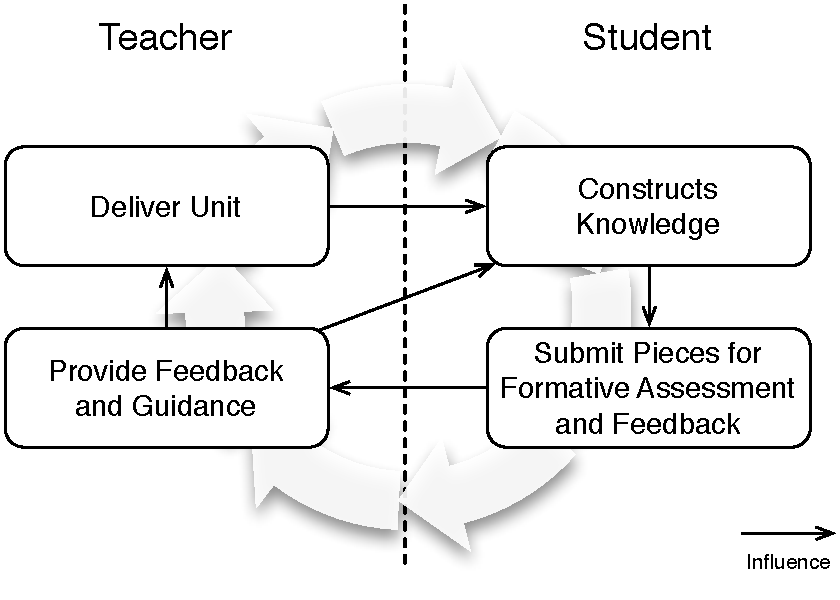
\includegraphics[width=2.5in]{DeliveryProcess}
	\caption{Iterative nature of the delivery process}
	\label{fig:delivery_overview}
\end{figure}

One critical aspect in our model is the iterative use of \emph{formative} feedback to help students construct appropriate knowledge, and to address misconceptions, as shown in \fref{fig:delivery_overview}. Teaching staff deliver teaching and learning activities to help students construct knowledge. These activities give students opportunities to create potential portfolio pieces that demonstrate their understanding. These pieces are submitted for feedback, that then inform future activities and provide students with advice they can use to help them address misconceptions, or otherwise improve their work.

The following principles were developed and used to guide the planning and delivery of teaching and learning activities:

\begin{itemize}
  \item Provide opportunities through activity design to actively engage students -- \emph{it is what the student does that counts}.  
  \item Relate all activities to the objectives, providing students with opportunities to create evidence for their portfolio.
  \item Use ungraded formative feedback to aid knowledge construction, with preference for small, frequent guidance.
\end{itemize}

In the example unit we avoided the use of traditional lecture style presentations, and included constructivist activities such as interactive presentations using audience response systems, role-plays, group design activities, and code walkthroughs. 

Students developed a number of programs based on constructive activities including a sort visualisation program (to introduce language constructs), a shape drawing program (to explore objects and inheritance), and a board game (to learn about object design and implementation for a larger problem).

% subsection the_role_of_formative_feedback (end)

\subsection{Constructing and Assessing Portfolios} % (fold)
\label{sub:assessing_the_portfolios}

The final phase of the process is the development and submission of portfolios by students, and assessment by staff. This process uses the outcomes and assessment criteria to determine what needs to be demonstrated and assessed. 

A number of papers discuss portfolio assessment for introductory programming units. Plimmer reports the successful use of portfolio assessment in an introductory programming unit in~\cite{Plimmer:2000}, where the portfolio contributed between 25\% and 60\% of the students' final grades. Programming portfolios were also discussed by Jones in~\cite{Jones:2010}, where students submitted a number of portfolio assignments during the semester. In both cases the portfolio was a collection of programs that were marked and contributed to a final grade.

Our proposed assessment model uses 100\% portfolio assessment. Formative feedback allows students to improve their understanding during delivery, without penalty for demonstrating their misunderstandings. The final portfolio then includes a student's best work, encouraging them to incorporate the feedback they receive. This is a highly considered position based on our own experience in prior units. Graded assessment during unit delivery encourages students to ``cover up'' their lack of knowledge or shallow understanding. Surely it must be the final outcomes that matter, not the rate of progress. With this in mind the common use of mid-term summative assessment is surprising.

% The use of an interview, or hurdle\footnote{In this case the hurdle test must be ``passed'' to pass the unit, but did not contribute to the final grade.} test, to help address plagiarism and increase confidence that the work in the portfolio is the students own work.

Based on our experience we suggest the following principles be used to guide the creation and assessment activities of portfolios:

\begin{itemize}
  \item Encourage unique, diverse, concise, and strongly aligned evidence.
  \item Motivate students to include evidence of learning from formative experience.
  \item Accurately and consistently follow the terms of the assessment criteria, as this is the \emph{contract} the students work towards.
  \item Require students to reflect on their learning, and the evidence in their portfolio, with respect to the intended learning outcomes of the unit and the assessment criteria.
  \item Use an interview, or hurdle\footnote{In this case the hurdle test must be ``passed'' to pass the unit, but did not contribute to the final grade.} test, to check minimal pass criteria in an invigilated manner. Where tests are used they need only distinguish between pass and fail, and do not need to address higher grades. 
\end{itemize}

Portfolios in the example unit were required to include a \emph{reflective report}, a \emph{hurdle test}, and additional pieces to demonstrate coverage of the learning outcomes. Students were encouraged to incorporate feedback they received during the delivery, and to include a range of pieces such as programs, reports, and concept maps. The hurdle test covered all basic content, and students had to demonstrate a good understanding of the principles covered in the unit, as well as sufficient programming proficiency. Where students failed the hurdle they were permitted to re-sit an equivalent test once.

% subsection assessing_the_portfolios (end)

% section process_details (end)

% subsection design_assessment_criteria (end)

% section design (end)

% section model (end)


\section{Discussion and Conclusion}

This work presents a model for applying constructive alignment with portfolio assessment for teaching introductory programming, along with principles to help guide the development and delivery of such units. The model and principles presented have been applied to the delivery of a number of introductory programming units, with positive feedback from students and staff. The initial implementation demonstrated the potential of the approach, with the model appearing to be worth further investigation, but the delivery requiring some adjustments. 

Students responded positively to the unit delivery as evidenced by the results in the university's student feedback on teaching survey. An additional survey was conducted to collect details on students approaches to learning, and their perceptions of the portfolio assessment. Only 16 students completed the survey with all comments being positive, as a quote from one student shows: 

\begin{quote}
  ``The portfolio was a great exercise, it stimulated me to do independent research and think about what I had learnt''   
\end{quote}

There were some challenges for staff related to a perceived \emph{loss of control}, \emph{via} vexation, with less motivated students not making the most of the formative opportunities. The unit had a lower than desired submission rate, with 64 portfolios being submitted from the initial enrolment of 83 students. Students achieved grades that indicate that the learning activities aligned with the outcomes, and interestingly resulted in an even distribution across the grade spectrum.

Future publications will examine the implementation of this model more fully; looking in more detail at the portfolios submitted, student approaches to learning, and possible adjustments to the model and principles in light of this analysis.


% chapter approaching_constructive_alignment_with_portfolio_assessment (end)